% This is samplepaper.tex, a sample chapter demonstrating the
% LLNCS macro package for Springer Computer Science proceedings;
% Version 2.20 of 2017/10/04
%
\documentclass[runningheads]{llncs}
%
\usepackage{graphicx}
% Used for displaying a sample figure. If possible, figure files should
% be included in EPS format.
%
% If you use the hyperref package, please uncomment the following line
% to display URLs in blue roman font according to Springer's eBook style:
% \renewcommand\UrlFont{\color{blue}\rmfamily}

\begin{document}
%
\title{Sparse-Matrix based Kernels for Expediting Quantum Neural Networks on Hardware Accelerators}
%
%\titlerunning{Abbreviated paper title}
% If the paper title is too long for the running head, you can set
% an abbreviated paper title here
%
\author{First Author\inst{1}\orcidID{0000-1111-2222-3333} \and
Second Author\inst{2,3}\orcidID{1111-2222-3333-4444} \and
Third Author\inst{3}\orcidID{2222--3333-4444-5555}}
%
\authorrunning{F. Author et al.}
% First names are abbreviated in the running head.
% If there are more than two authors, 'et al.' is used.
%
\institute{Princeton University, Princeton NJ 08544, USA \and
Springer Heidelberg, Tiergartenstr. 17, 69121 Heidelberg, Germany
\email{lncs@springer.com}\\
\url{http://www.springer.com/gp/computer-science/lncs} \and
ABC Institute, Rupert-Karls-University Heidelberg, Heidelberg, Germany\\
\email{\{abc,lncs\}@uni-heidelberg.de}}
%
\maketitle              % typeset the header of the contribution
%
\begin{abstract}
The abstract should briefly summarize the contents of the paper in
15--250 words.

\keywords{First keyword  \and Second keyword \and Another keyword.}
\end{abstract}
%
%
%
\section{Introduction}

Researchers have applied Deep Neural Networks (DNN) \cite{Hinton} to a range of scientific and societal applications, which includes deploying text and speech recognition systems and exploring the vast unknown frontiers of science. Loosely modeled after the complex structure of a biological learning system, DNNs derive an input-output mapping, through an interconnected set of nodes. Even though substaintial strides have been taken in reducing the computational expense of training a DNN, researchers have often incorporated concepts from different fields to ascend barriers. For example, expediting matrix computations on hardware accelerators is insipred from the field of algorithm-hardware co-design; replacing backpropagation algorithm with genetic algorithm for DNN optimization is an idea drawn from natrual meta-heuristics. 

With the advent of Quantum Computing (QC), integrating the main components of QC with DNNs is an extremely exciting avenue. The electic combination of quantum mechanics with neural computation gave rise to Quantum Neural Network models (QNN) \cite{Kak} \cite{Chrisley}. The motivation behind developing QNNs is to circumvent the limitations faced by classic DNNs in handling complex unstructured datasets by resorting to features of quantum entanglement, superposition and unitary transformations. The work done in developing QNNs has revolved around generalizing the perceptron structure and the associated activation function, as the classical representations resist the mathematical formulation of quantum mechanics \cite{steck}. The principle theoretical challenge faced in QNN development is the linear nature of quantum processes which is a hurdle as majority of the networks have a crucial dependence on non-linear activation functions. Despite such complications, QNNs present a enticing approach to develop large scale networks with reduced computational expense.

The latency observed when a QNN is subjected to large volumes of datasets contributes to sustaintial overhead. The main technique employed to reduce inference latency for DNNs is to prune the network, which transforms the dense network to a sparse model by trimming off network connections which reduce the model accuracy. However, there exists a trade-off between the amount of sparsity introduced in a network and model validity. Researchers have dwelled on the level of fine tunning must be applied, which element-wise pruning\cite{Han} being the most granular and sparsity pattern being the least granular\cite{Han2}.    

To accelerate the sparse QNN, the core computations are ported onto accelerator platforms like GPUs and FPGAs. The hardware architecture of these accelerators is radically different from a CPU architecture, which emphasis placed on data crunching rather than accomodating multiple tasks.  GPUs have multiple multiprocessors, each of which has multiple Streaming Processors (SM) organized into blocks, having larger globally shared memory rather than locally shared memory. Organizing these blocks along with shared memory offers ultra fine-tuned task and data parallelism, resulting in high throughput and bottleneck elimination.   
\subsection{A Subsection Sample}
Please note that the first paragraph of a section or subsection is
not indented. The first paragraph that follows a table, figure,
equation etc. does not need an indent, either.

Subsequent paragraphs, however, are indented.

\subsubsection{Sample Heading (Third Level)} Only two levels of
headings should be numbered. Lower level headings remain unnumbered;
they are formatted as run-in headings.

\paragraph{Sample Heading (Fourth Level)}
The contribution should contain no more than four levels of
headings. Table~\ref{tab1} gives a summary of all heading levels.

\begin{table}
\caption{Table captions should be placed above the
tables.}\label{tab1}
\begin{tabular}{|l|l|l|}
\hline
Heading level &  Example & Font size and style\\
\hline
Title (centered) &  {\Large\bfseries Lecture Notes} & 14 point, bold\\
1st-level heading &  {\large\bfseries 1 Introduction} & 12 point, bold\\
2nd-level heading & {\bfseries 2.1 Printing Area} & 10 point, bold\\
3rd-level heading & {\bfseries Run-in Heading in Bold.} Text follows & 10 point, bold\\
4th-level heading & {\itshape Lowest Level Heading.} Text follows & 10 point, italic\\
\hline
\end{tabular}
\end{table}


\noindent Displayed equations are centered and set on a separate
line.
\begin{equation}
x + y = z
\end{equation}
Please try to avoid rasterized images for line-art diagrams and
schemas. Whenever possible, use vector graphics instead (see
Fig.~\ref{fig1}).

\begin{figure}
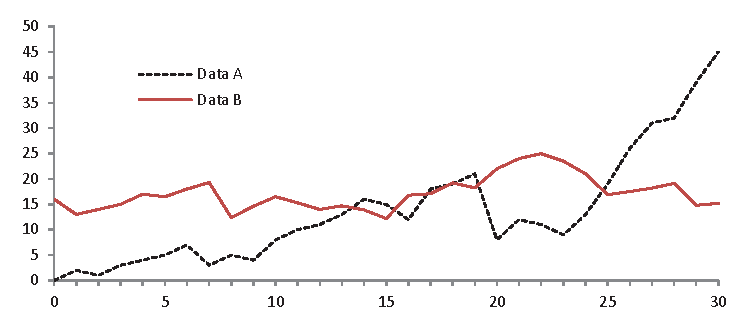
\includegraphics[width=\textwidth]{fig1.eps}
\caption{A figure caption is always placed below the illustration.
Please note that short captions are centered, while long ones are
justified by the macro package automatically.} \label{fig1}
\end{figure}

\begin{theorem}
This is a sample theorem. The run-in heading is set in bold, while
the following text appears in italics. Definitions, lemmas,
propositions, and corollaries are styled the same way.
\end{theorem}
%
% the environments 'definition', 'lemma', 'proposition', 'corollary',
% 'remark', and 'example' are defined in the LLNCS documentclass as well.
%
\begin{proof}
Proofs, examples, and remarks have the initial word in italics,
while the following text appears in normal font.
\end{proof}
For citations of references, we prefer the use of square brackets
and consecutive numbers. Citations using labels or the author/year
convention are also acceptable. The following bibliography provides
a sample reference list with entries for journal
articles~\cite{ref_article1}, an LNCS chapter~\cite{ref_lncs1}, a
book~\cite{ref_book1}, proceedings without editors~\cite{ref_proc1},
and a homepage~\cite{ref_url1}. Multiple citations are grouped
\cite{ref_article1,ref_lncs1,ref_book1},
\cite{ref_article1,ref_book1,ref_proc1,ref_url1}.
%
% ---- Bibliography ----
%
% BibTeX users should specify bibliography style 'splncs04'.
% References will then be sorted and formatted in the correct style.
%
% \bibliographystyle{splncs04}
% \bibliography{mybibliography}
%
\begin{thebibliography}{8}
\bibitem{Hinton}
Hinton, G. E., Osindero, S. and Teh, Y.
A fast learning algorithm for deep belief nets.
Neural Computation 18, pp 1527-1554.

\bibitem{Kak}
Kak, S. (1995). "On quantum neural computing". Advances in Imaging and Electron Physics. 94: 259–313. doi:10.1016/S1076-5670(08)70147-2. ISBN 9780120147366.

\bibitem{Chrisley}
Chrisley, R. (1995). "Quantum Learning". In Pylkkänen, P.; Pylkkö, P. (eds.). New directions in cognitive science: Proceedings of the international symposium, Saariselka, 4–9 August 1995, Lapland, Finland. Helsinki: Finnish Association of Artificial Intelligence. pp. 77–89. ISBN 951-22-2645-6.

\bibitem{steck}
Behrman, E. C., Steck, J. E., Kumar, P., \& Walsh, K. A. Quantum Algorithm design using dynamic learning. Quantum Information and Computation. 2008, 8(1\&2),12–29.

\bibitem{Han}
S. Han, J. Pool, J. Tran, and W. Dally, “Learning both weights
and connections for efficient neural network,” in Advances in neural
information processing systems, 2015, pp. 1135–1143.

\bibitem{Han2}
S. Han, X. Liu, H. Mao, J. Pu, A. Pedram, M. A. Horowitz, and
W. J. Dally, “Eie: Efficient inference engine on compressed deep
neural network,” in Proceedings of the 43rd International Symposium
on Computer Architecture, ser. ISCA 16. IEEE Press, 2016, p. 243254.
[Online]. Available: https://doi.org/10.1109/ISCA.2016.30
\bibitem{ref_url1}
LNCS Homepage, \url{http://www.springer.com/lncs}. Last accessed 4
Oct 2017
\end{thebibliography}
\end{document}
